% NEUTRONICS BEAMER TEMPLATE -- START EDITING IN LINE 90
\documentclass[xcolor=x11names, compress, handout]{beamer}
%\documentclass[xcolor=x11names, compress]{beamer}
\usepackage{pgfpages}
\usepackage{algorithm}
\usepackage{algpseudocode}
\usepackage{appendixnumberbeamer}
\usepackage{booktabs}
\usepackage{amsmath}
\usepackage{tikz}
\usepackage{xcolor}
\usepackage[super]{nth}
\usepackage{sty/commands}
\usepackage{appendixnumberbeamer}
\usepackage{hyperref}
\usepackage{listing}
% \usepackage{array}


\definecolor{CoolBlack}{rgb}{0.0, 0.18, 0.39}
\definecolor{byellow}{rgb}{0.55037, 0.38821, 0.06142}

\usetikzlibrary{decorations.fractals}

\setbeamerfont{title like}{shape=\scshape}
\setbeamerfont{frametitle}{shape=\scshape}

\setbeamercolor*{lower separation line head}{bg=CoolBlack}
\setbeamercolor*{normal text}{fg=black,bg=white}
\setbeamercolor*{alerted text}{fg=dgreen} 
\setbeamercolor*{example text}{fg=black}
\setbeamercolor*{structure}{fg=black}

\setbeamertemplate{bibliography item}{\insertbiblabel}
% Margins
\mode<presentation>
{
  % \definecolor{berkeleyblue}{HTML}{003262}
  % \definecolor{berkeleygold}{HTML}{FDB515}
  \definecolor{berkeleyblue}{HTML}{FF8200}
  \definecolor{berkeleygold}{HTML}{808080}
  \usetheme{Boadilla}      % or try Darmstadt, Madrid, Warsaw, Boadilla...
  % \usecolortheme{dove} % or try albatross, beaver, crane, ...
  \setbeamercolor{structure}{fg=berkeleyblue,bg=berkeleygold}
  \setbeamercolor{palette primary}{fg=berkeleyblue,bg=berkeleygold}
  \setbeamercolor{palette secondary}{fg=berkeleyblue,bg=berkeleygold}
  \setbeamercolor{palette tertiary}{bg=berkeleyblue,fg=white}
  \usefonttheme{structurebold}  % or try serif, structurebold, ...
  \useinnertheme{circles}
  \setbeamertemplate{caption}[numbered]
  \usebackgroundtemplate{}
}

%% Beamer Layout %%%%%%%%%%%%%%%%%%%%%%%%%%%%%
\useoutertheme[subsection=false,shadow]{miniframes}
%\useinnertheme{default}
%\usefonttheme{serif}
%\usepackage{palatino}
%\usepackage{tabu}
% addition of color
\definecolor{dgreen}{rgb}{0.,0.6,0.}
\definecolor{RawSienna}{cmyk}{0,0.72,1,0.45}
%\usepackage[sorting=none]{biblatex}
\mode<presentation>

% Links
\definecolor{links}{HTML}{003262}
\hypersetup{colorlinks,linkcolor=,urlcolor=links}

% columns
\renewcommand{\(}{\begin{columns}}
\renewcommand{\)}{\end{columns}}
\newcommand{\<}[1]{\begin{column}{#1}}
\renewcommand{\>}{\end{column}}


% Show table of content before each section
\AtBeginSection[]{
  \AtBeginSection[]{
  \begin{frame}[noframenumbering, plain]
  \frametitle{Outline}                     
  \centering
  \begin{minipage}[t][0.5\textheight]{0.75\textwidth}
    \linespread{2.0}
    \tableofcontents[currentsection]
  \end{minipage}
  \end{frame}
  }
}

% 
%THIS IS THE TITLE OF THE TALK
\title{GEANT4 Simulations}

%FEEL FREE TO EDIT THE COVER LAYOUT AS NEEDED
\author{Su-Ann Chong}

\date{July \nth{31}, 2020}


\begin{document}

\begin{frame}[plain]
  %THIS IS THE TITLE OF THE TALK
  \title{NE 697: \\\large{GEANT4 Simulations of Light Transport in \\
  $^6$Li Glass Scintillator}}

  %FEEL FREE TO EDIT THE COVER LAYOUT AS NEEDED
  \author{Su-Ann Chong}
  % \institute{Monthly Group Meeting}
  % \institute{University of Tennessee, Knoxville/ Nuclear Engineering Department}
  \date{July \nth{31}, 2020}
  \titlepage
\end{frame}

%----------------------------------------------------------%
% WHEN YOU START A NEW SECTION, IT WILL SHOW UP AS A CLICKABLE
% SHORTCUT AT THE TOP OF YOUR FRAMES

\begin{frame}
  \frametitle{Outline}
  %\hfill                        
  \centering
  \begin{minipage}[t][0.5\textheight]{0.75\textwidth}
   \linespread{2.0}
   \tableofcontents
   \vfill
 \end{minipage}
  % \parbox{0.73\textwidth}{
  %   \tableofcontents
  %   }
\end{frame}


\section{\scshape Introduction}
\begin{frame}
  \frametitle{Introduction}
  \begin{columns}
  \begin{column}{0.6\textwidth}
  Understanding and optimizing light collection is critical for achieving high performance in scintillation detectors. \\
  \ \\
  The light transport in the crystal is dependent on 
  \begin{itemize}
  \item the crystal geometry, 
  \item the bulk absorption and scattering of the material, 
  \item the surface treatment of the crystal faces. 
  \end{itemize}
  \ \\
  \end{column}
  \begin{column}{0.3\textwidth}
  \begin{center}
  % \begin{figure}
  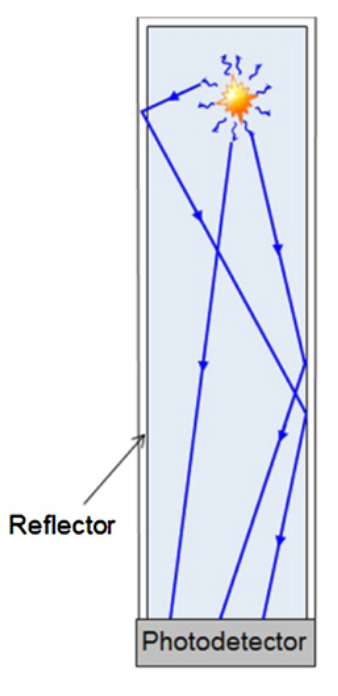
\includegraphics[scale=0.5]{images/scintillation.png}
  \scriptsize Reflection of optical photons within a scintillator. Image obtained from \cite{roncali_cherry_2013}.
  % \end{figure}
  \end{center}
  \end{column}
  \end{columns}

\end{frame}

\begin{frame}
\frametitle{GEANT4 Surface Treatment Models  }
\scriptsize 
\begin{itemize}
\item glisur (GEANT3) \\
Users indicate the value of polish, where a random point is generated in a sphere of radius (1-polished), and the corresponding vector is added to the average surface nominal normal as the micro-facet normal. A specular reflection is thereafter calculated based on the microfacet orientation. \cite{geant4_doc} \cite{janecek_moses_2010} \\
\ \\

\item unified\\
 Users specify a parameter $SigmaAlpha$, which defines the standard deviation of the Gaussian distribution of micro-facets around the average surface normal. \cite{geant4_doc} Four kinds of surface reflections are possible: specular, spike, lobe, backscatter and Lambertian. \cite{janecek_moses_2010} \\
 \ \\

 Note: Geant4 assumes that the four reflection type probabilities are constants, and not functions of incidence angles, which does not fully agree with measured data in Ref. \cite{janecek_moses_2010} \\
 \ \\

 % The probability of micro-facet normals populates the annulus of solid angle $sin(\alpha) d\alpha$ will be proportional to a gaussian of $SigmaAlpha$
\item LUT \\
Model is based on measured surface data with rough and polished finishes that can be coupled without reflectors, or in combination with a specular reflector (e.g. ESR) or a Lambertian reflector (e.g. Teflon). Coupling method can be air or optical grease. \cite{geant4_doc}
\end{itemize}
\end{frame}

\begin{frame}
\frametitle{Types of Reflection}


\begin{columns}
\begin{column}{0.4\textwidth}
\scriptsize
Surface reflections components: \\
\centering
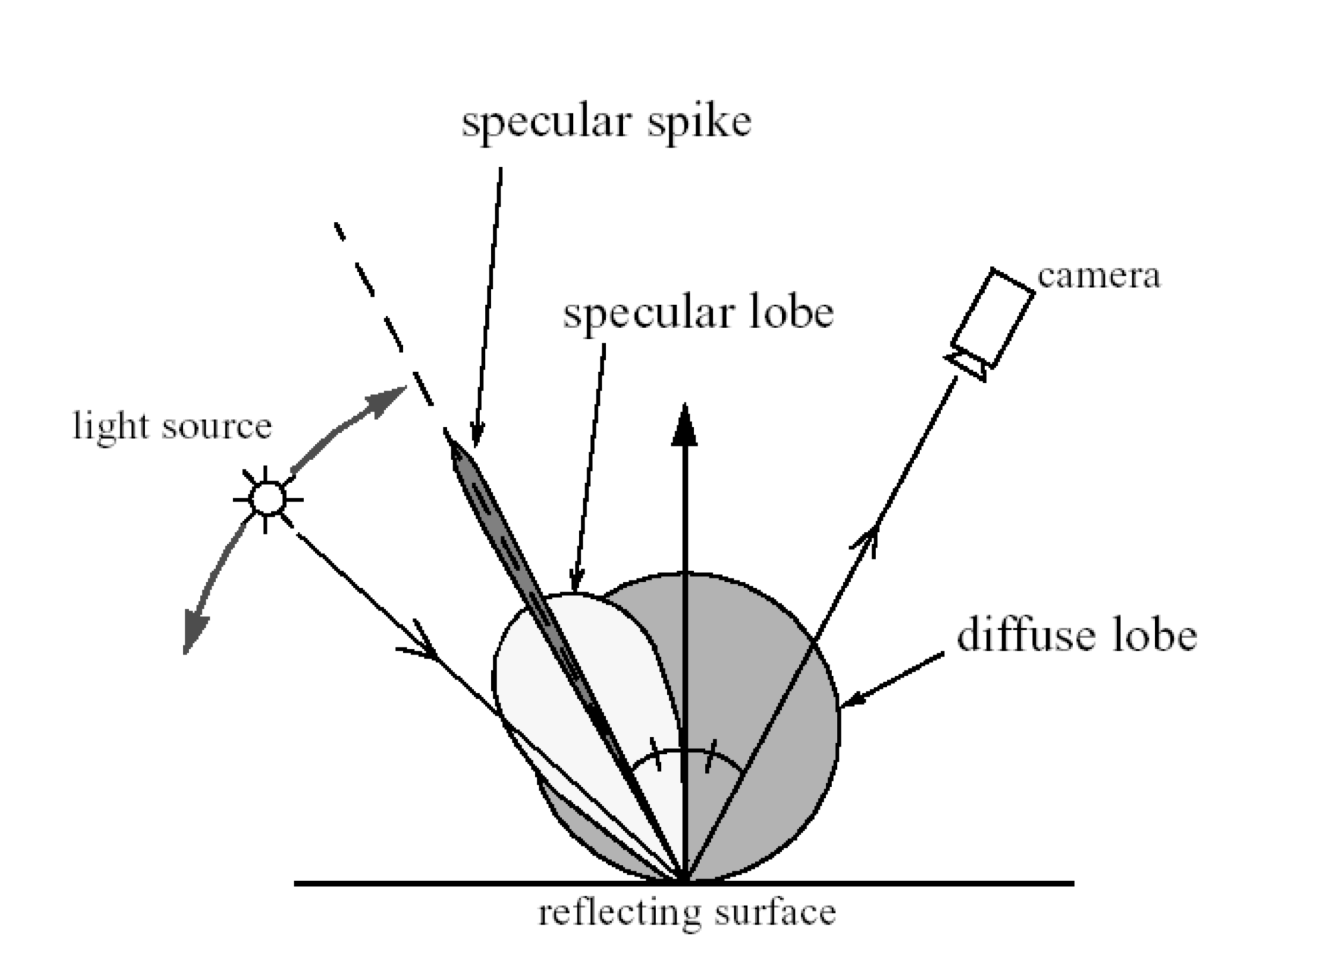
\includegraphics[width=\textwidth]{images/surface_reflection.png}
% \scriptsize
% \begin{block}{Note}
% % Unified model requires users to sepecify 4 reflection probability distributions, namely specular lobe, specular spike, backscatter and reflectivity.  
% Specular spike: the reflected photon is reflected about the average surface normal \\
% Backscatter: the photon is reflected by into the direction the photon came from \\
% Lambertian: the photon will be reflected with a Lambertian distribution (cosine distribution) about the average surface normal \\
% Specular lobe: the surface is assumed to consist of micro-facets, which are oriented around the average surface with a Gaussian distribution defined by $SigmaAlpha$. A micro-facet is randomly selected from the distribution defined by $SigmaAlpha$, and a specular reflection is thereafter calculated based on the micro-facet orientation. 
% \end{block}

\end{column}
\begin{column}{0.6\textwidth}
\scriptsize
\begin{block}{Terminology \cite{janecek_moses_2010}}
% Unified model requires users to sepecify 4 reflection probability distributions, namely specular lobe, specular spike, backscatter and reflectivity.  
\begin{tabular}{c p{4.5cm}}
Specular spike & the reflected photon is reflected about the average surface normal \\
Backscatter & the photon is reflected by into the direction the photon came from \\
Lambertian & the photon will be reflected with a Lambertian distribution (cosine distribution) about the average surface normal \\
Specular lobe & the surface is assumed to consist of micro-facets, which are oriented around the average surface with a Gaussian distribution defined by $SigmaAlpha$. A micro-facet is randomly selected from the distribution defined by $SigmaAlpha$, and a specular reflection is thereafter calculated based on the micro-facet orientation. 
\end{tabular}
\end{block}
% Specular
% 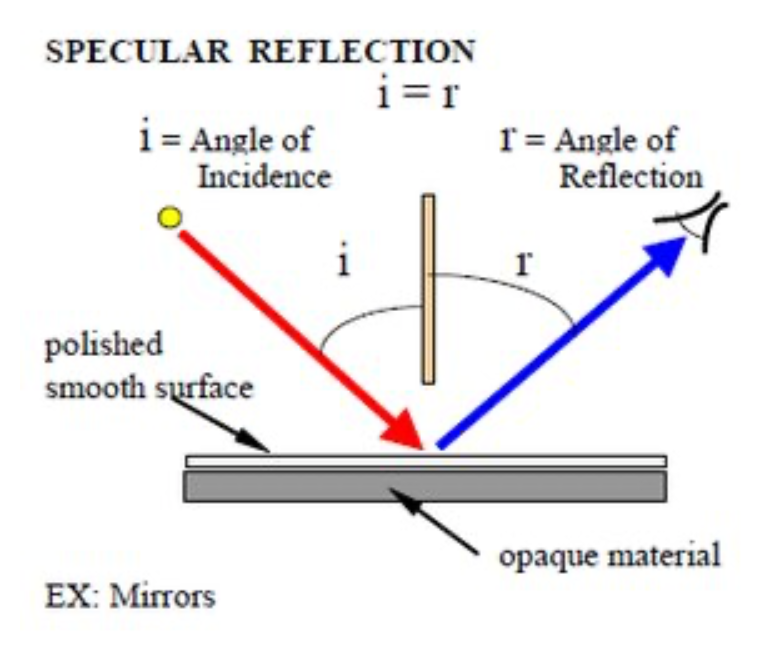
\includegraphics[width=0.8\textwidth]{images/specular.png}
% Lambertian
% 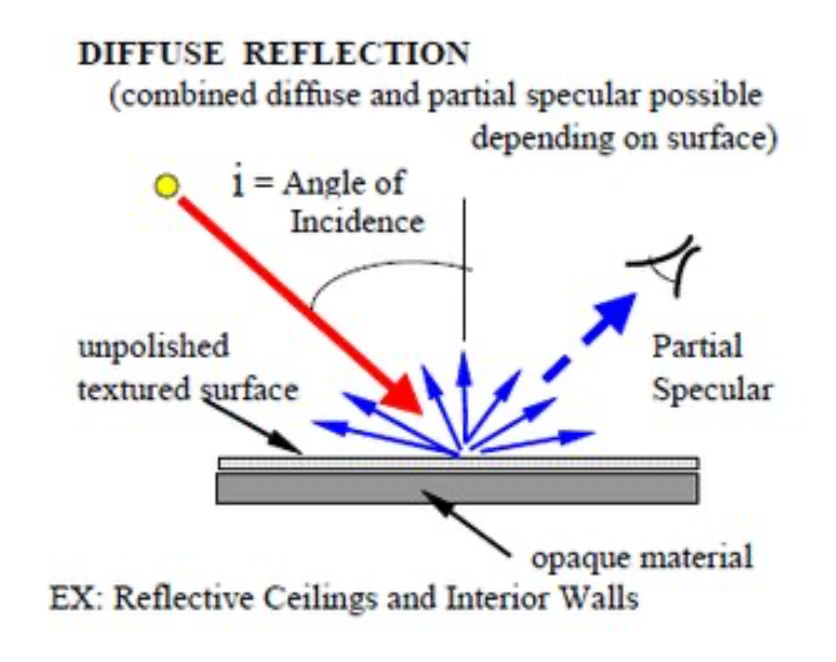
\includegraphics[width=0.8\textwidth]{images/lambertian.png}
\end{column}
\end{columns}
\end{frame}

\begin{frame}
\frametitle{Micro-Facets}
\centering
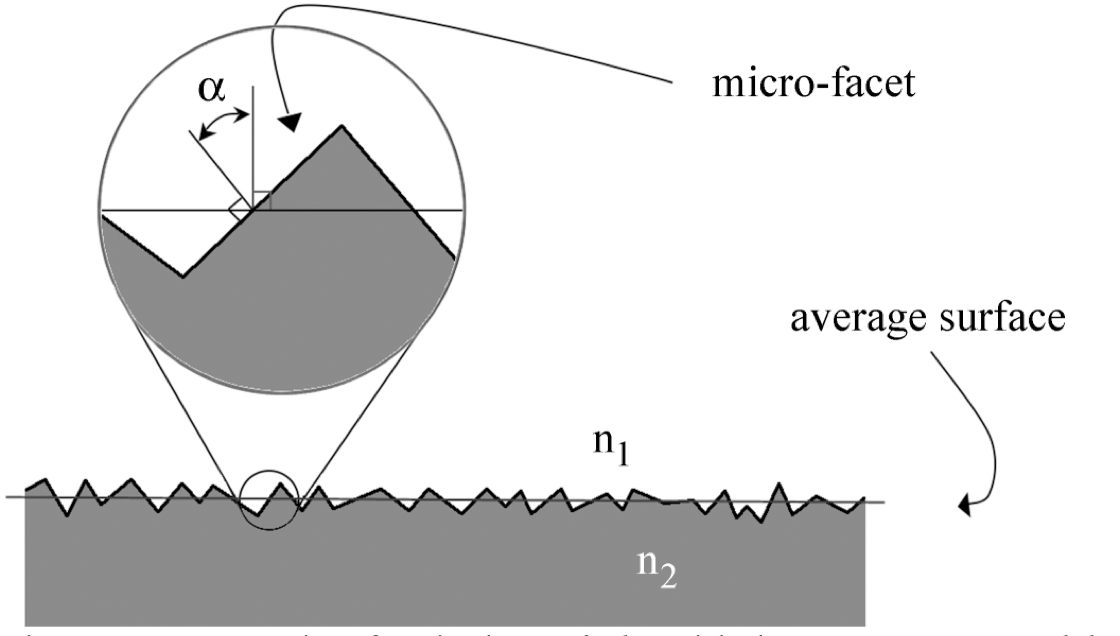
\includegraphics[width=0.6\textwidth]{images/microfacets.png}
\scriptsize \\
For a ground surface in the unified model, the parameter $SigmaAlpha$ defines the standard deviation of the Gaussian distribution of micro-facets around the average surface normal. \\ Image obtained from \cite{janecek_moses_2010}.

\begin{block}{Note}
Optical Monte Carlo software such as DETECT, Litrani, Geant4 or GATE allow the operator to set the surface reflections as purely specular, purely diffuse (Lambertian), or a linear combination of specular and Lambertian, which might not be a true representation of the real world. \cite{janecek_moses_2008}\\
\hfill  - Janecek, 2008
\end{block}
\end{frame}


\section{\scshape Simulation Model}
\begin{frame}
\frametitle{GEANT4 Simulation Model}
Goals:
\begin{itemize}
\item Light collection efficiency based on crystal geometry, surface finish, reflector type and coupling method.
\item Light sharing of monolithic and pixelated scintillators across array of photodetectors
\end{itemize}
\ \\
\ \\
Key Model Parameters:
\begin{itemize}
\item Source: monoenergetic neutron beam at 25 meV (1.8 \AA) 
\item Geometry: single pixel and pixel array (8 $\times$ 8 pixels)
\item Material: $^6$Li-enriched glass scintillator (GS 20, Scintacor)
\item Physics list: $\leq$ 20 MeV neutron, G4OpticalPhysics 
% \item Output: ROOT files
\end{itemize}
\end{frame}

\begin{frame}
\frametitle{Primary particles}
Utilize a built-in primary particle generator $\rightarrow$ G4GeneralParticleSource: \\
\begin{columns}
\begin{column}{0.55\textwidth}

\begin{itemize}
\item Offers many pre-defined options 
  \begin{itemize}
  \item particle type \\ (neutron, gamma, proton, etc.)
  \item position distribution \\(point, plane, beam, etc.)
  \item angular distribution \\(isotropic, cosine-law, etc.)
  \item energy distributions \\(mono-energetic, power-law etc.)
  % \item multiple sources (user defined relative intensity) 
  \end{itemize}
\item Can be used via C++ or command line (or macro) UI
\end{itemize} 
\end{column}
\begin{column}{0.45\textwidth}
\begin{block}{Example GPS setup using macro}
$/gps/energy ~~0.025 ~eV$
$/gps/particle ~~neutron$
$/gps/direction ~~0. ~~0. ~~1.$
$/gps/pos/type ~~Beam$
$/gps/pos/shape ~~Circle$
$/gps/pos/sigma_r  ~~4 ~mm$ 
$/gps/pos/centre ~~0. ~~0. ~~-10. ~cm$
\end{block}
\end{column}
\end{columns}
\end{frame}

\begin{frame}
\frametitle{Detector Geometry}
Two detector geometry configurations: \\
\
\begin{columns}
\begin{column}{0.49\textwidth}
\centering
single pixel \\
\ \\
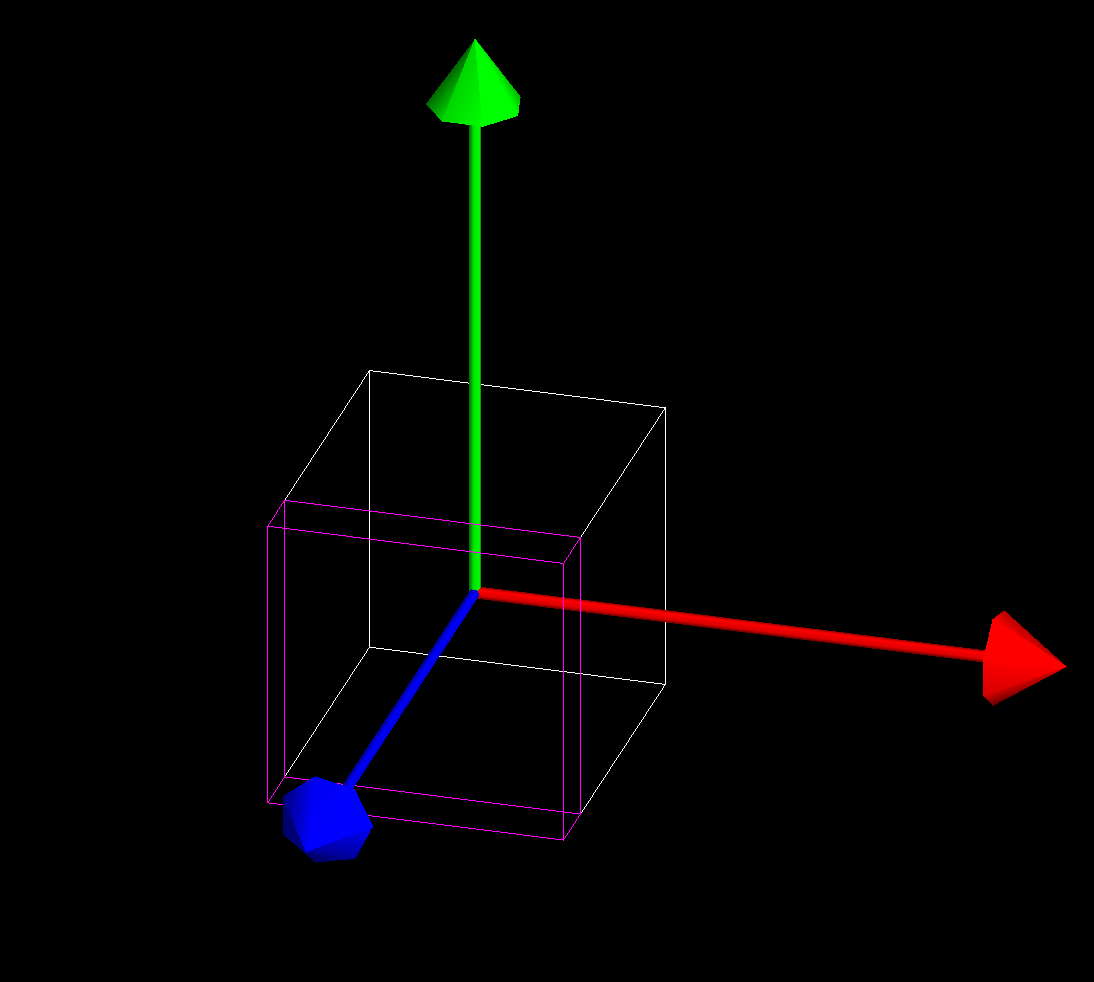
\includegraphics[width=\textwidth, height=5cm]{images/singlepixel.png}
\end{column}
\begin{column}{0.49\textwidth}
\centering
8 $\times$ 8 pixel array \\
\ \\
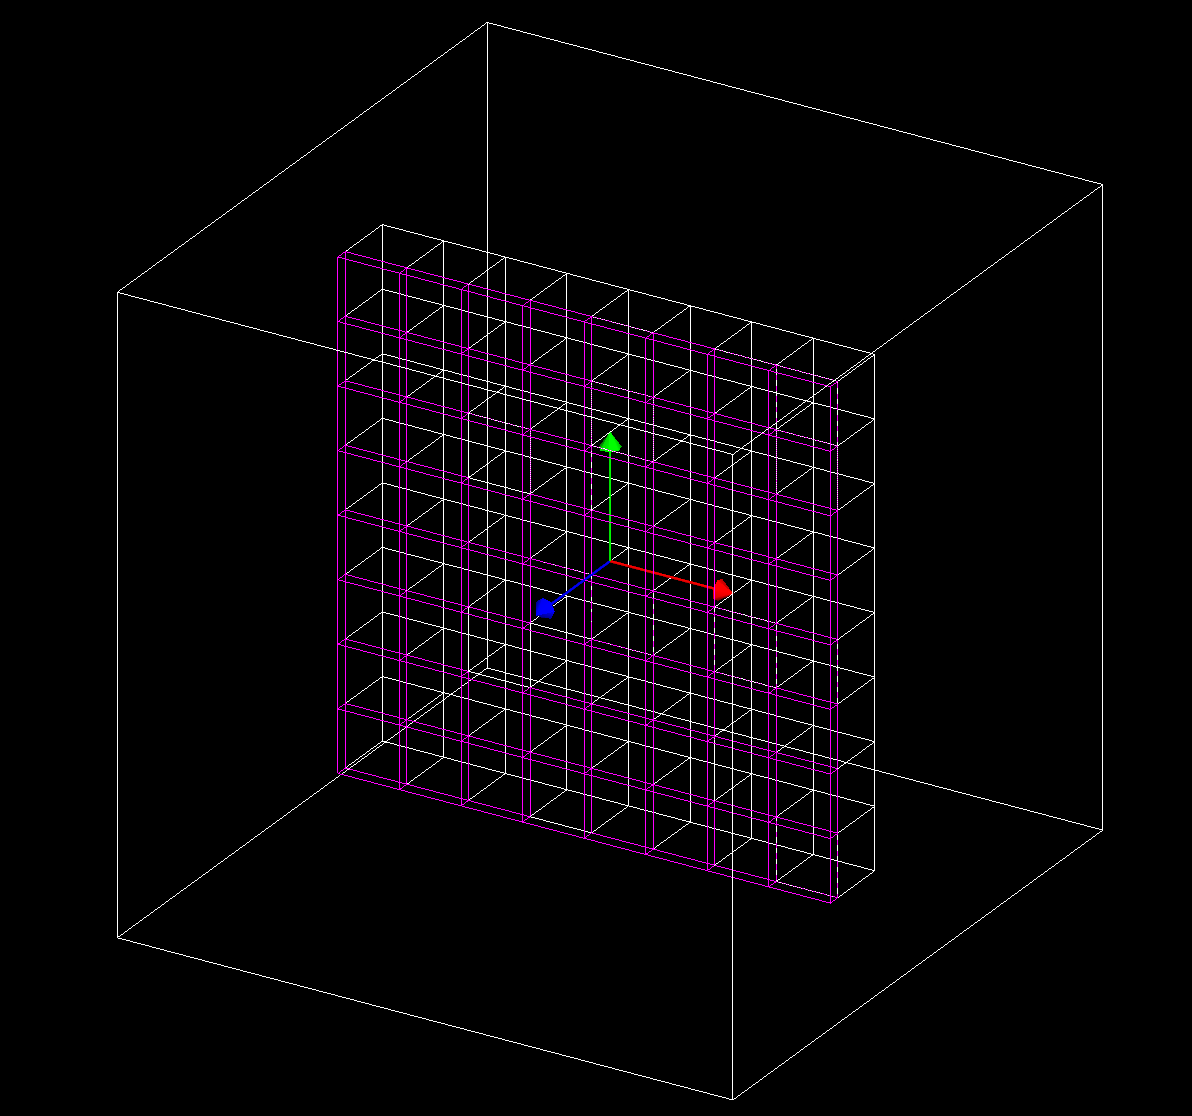
\includegraphics[width=\textwidth, height=5cm]{images/pixelarray.png}
\end{column}
\end{columns}
\ \\
\centering
scintillator (white wiring), photodetector (magenta wiring)
\end{frame}

\begin{frame}
\frametitle{Scintillator Material Composition and Properties}
\scriptsize
\begin{block}{Material Composition \cite{spowart_1976}}
\centering 
\begin{tabular}{p{1.7cm} | p{1.0cm} p{1.0cm} p{1.0cm} p{1.0cm} p{1.0cm} p{1.0cm} p{1.0cm}}
% \hline
 & SiO$_2$ & MgO & Al$_2$O$_3$ & Ce$_2$O$_3$ & Li$_2$O & Li & $^6$Li  \\
 \hline
Weight \% & 57 & 4 & 18 & 4 & 17.1 & 7.9 & 7.87 \\
% \hline
\end{tabular}
\end{block}
% \scriptsize \begin{center} Material composition of GS20 obtained from \cite{spowart_1976}. \end{center}

\begin{block}{Material Properties \cite{gs20}}
\centering \scriptsize
\begin{tabular}{c | c }
% \hline
Density (g/cm$^3$) & 2.50 \\
Wavelength$^\dagger$ (nm) & 395 \\
Refractive index$^\dagger$ & 1.55 \\
Decay time$^\ddagger$ (ns) & 18/57/98 \\
Scintillation yield$^{\dagger\dagger}$ (photons/MeV) &  \textasciitilde 1,276 \\
Linear attenuation coefficient$^{\ddagger\ddagger}$ (cm$^{-1}$) & 14.85 \\
Photon absorption length (cm) & 100 (assumed) \\
Yield ratio & 1.0 \\
Resoution scale & 1.0 \\
% \hline
\end{tabular}
\end{block}

\scriptsize  
$^\dagger$  at maximum emission. Full emission spectrum will be needed in simulation \\
$^\ddagger$ Fast component, slow component and 90\% to 10\% respectively \\
$^{\dagger\dagger}$ About 6,000 photons per absorbed neutron is normalized by the Q-value (4.73 MeV)\\
$^{\dagger\dagger}$ at thermal neutron energy (2meV) \\
% \begin{center}  Typical material properties of GS20 obtained from \cite{gs20}.  \end{center}

\end{frame}

\begin{frame}
\frametitle{Scintillator Boundary Interaction}
\scriptsize
% Parameters:
% \begin{itemize}
% \item Surface type 
% \item Optical surface mode 
% \item Optical surface finish 
% \end{itemize}

\begin{block}{Surface treatment}
\centering
\begin{tabular}{c | c }
% \hline
 surface type & dielectric-dielectric, dielectric-LUT $^\dagger$ \\
 &  dielectric-LUTDAVIS $^\ddagger$\\
 model &  unified, LUT, DAVIS   \\
 surface finish & rough, polished \\
 reflector type & teflon (lambertian), ESR (specular) \\
 coupling method & air \\
 crystal thickness & 1, 2, 6, 20 mm \\
 % \hline
\end{tabular}
\end{block}

$^\dagger$ LUT model is based on BGO crystal. \cite{janecek_moses_2008} \\
$^\ddagger$ DAVIS model is based on LYSO crystal \cite{roncali_cherry_2013} \\
% $^\dagger\dagger$ unified model

\begin{block}{Parameters for unified model}
\centering
\begin{tabular}{c | c}
$SigmaAlpha$  & 0.0227 rad/1.3$^o$ (polished) \\
& 0.209 rad / 12$^o$ (rough) \\
\end{tabular}
\end{block}
\end{frame}

\begin{frame}
\frametitle{Simulated Detector Setup}
\scriptsize \centering
single pixel (light collection efficiency) \\
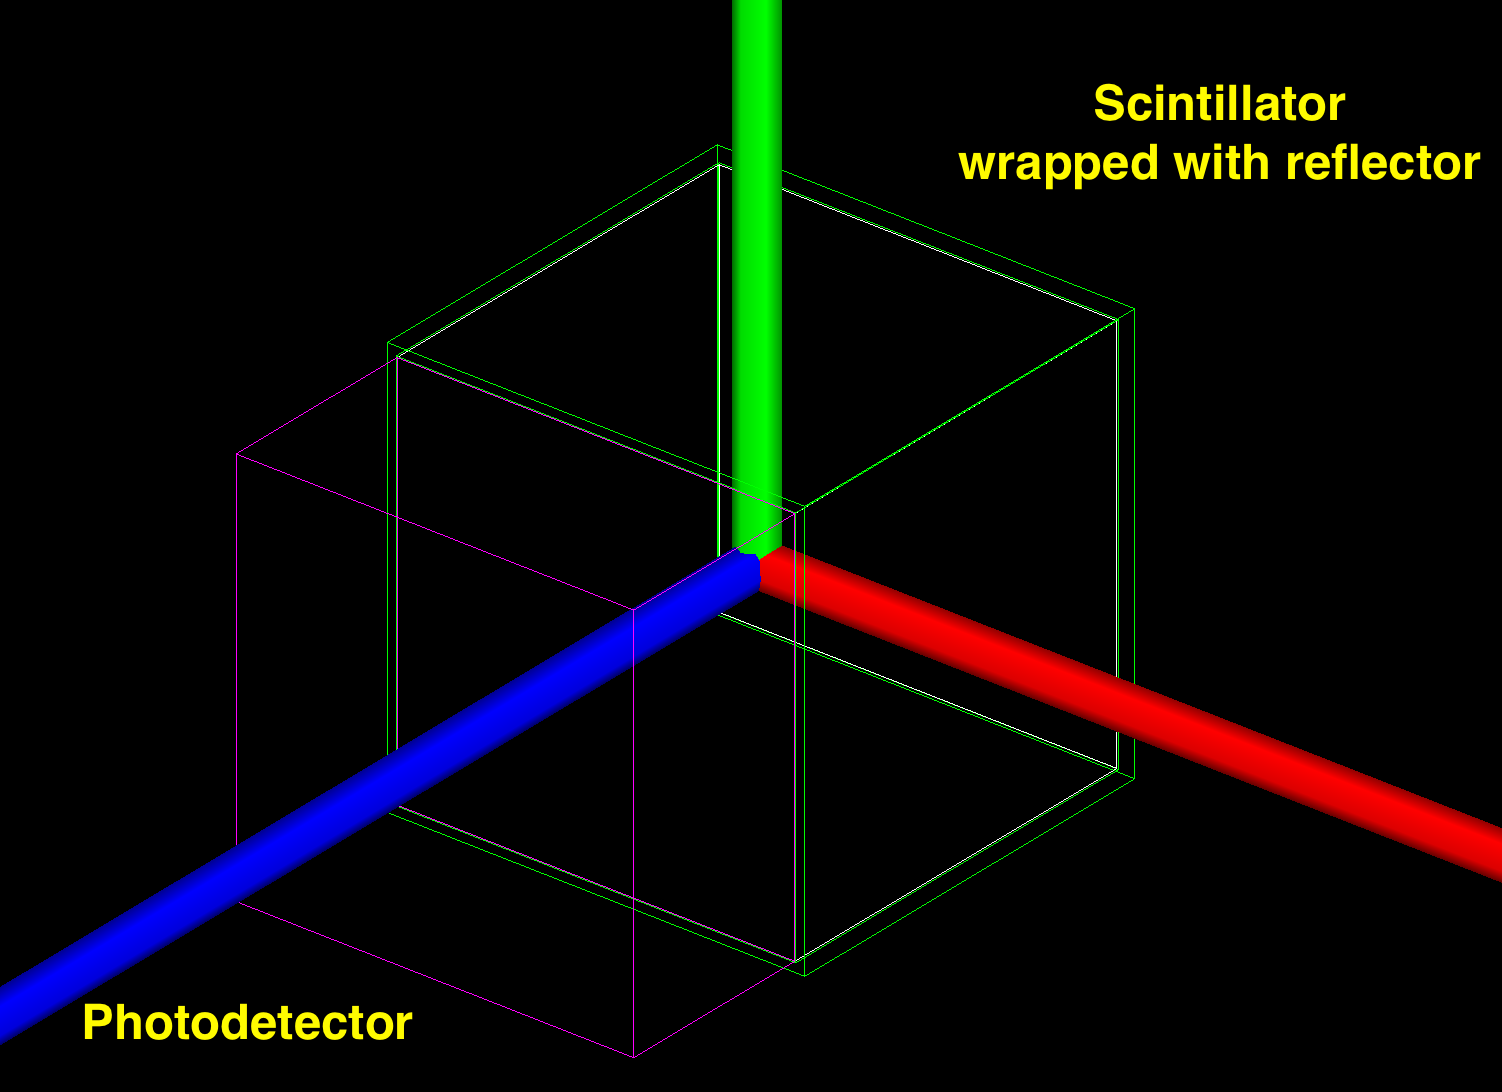
\includegraphics[width=0.48\textwidth, height=0.4\textheight]{images/scint_refl1.png}
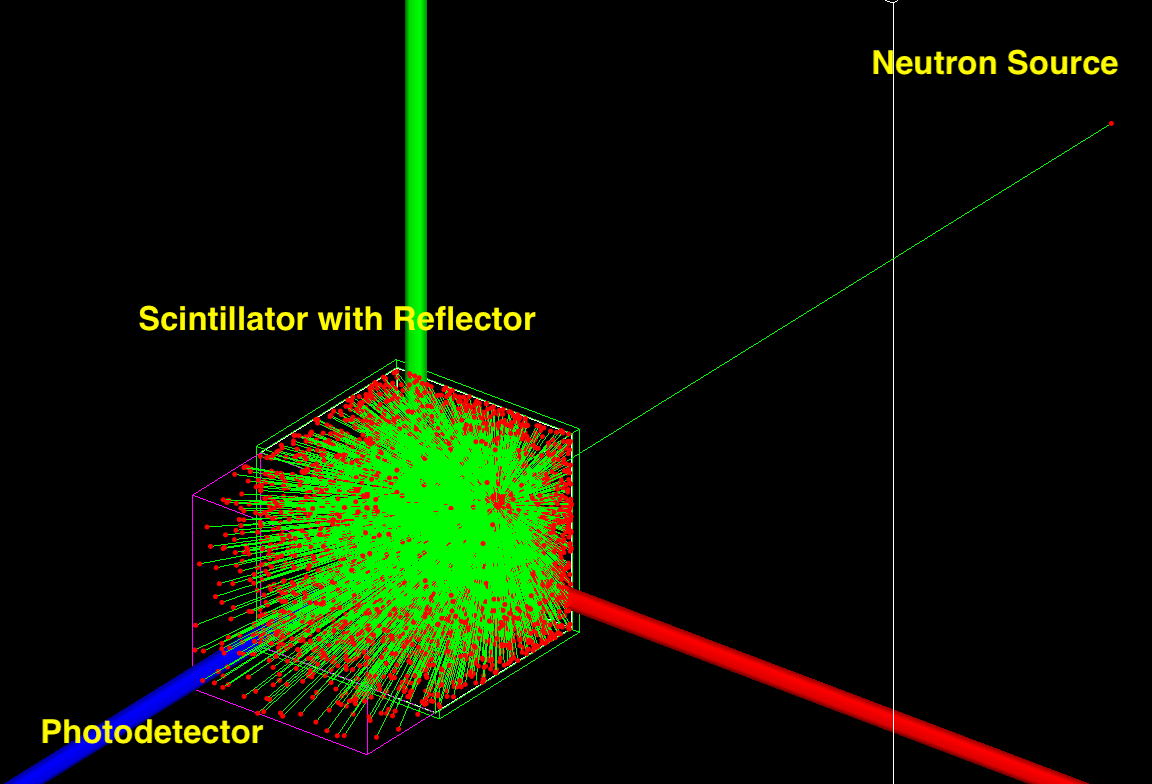
\includegraphics[width=0.48\textwidth, height=0.4\textheight]{images/scint_refl_neutron.png}
pixel array (light sharing)\\
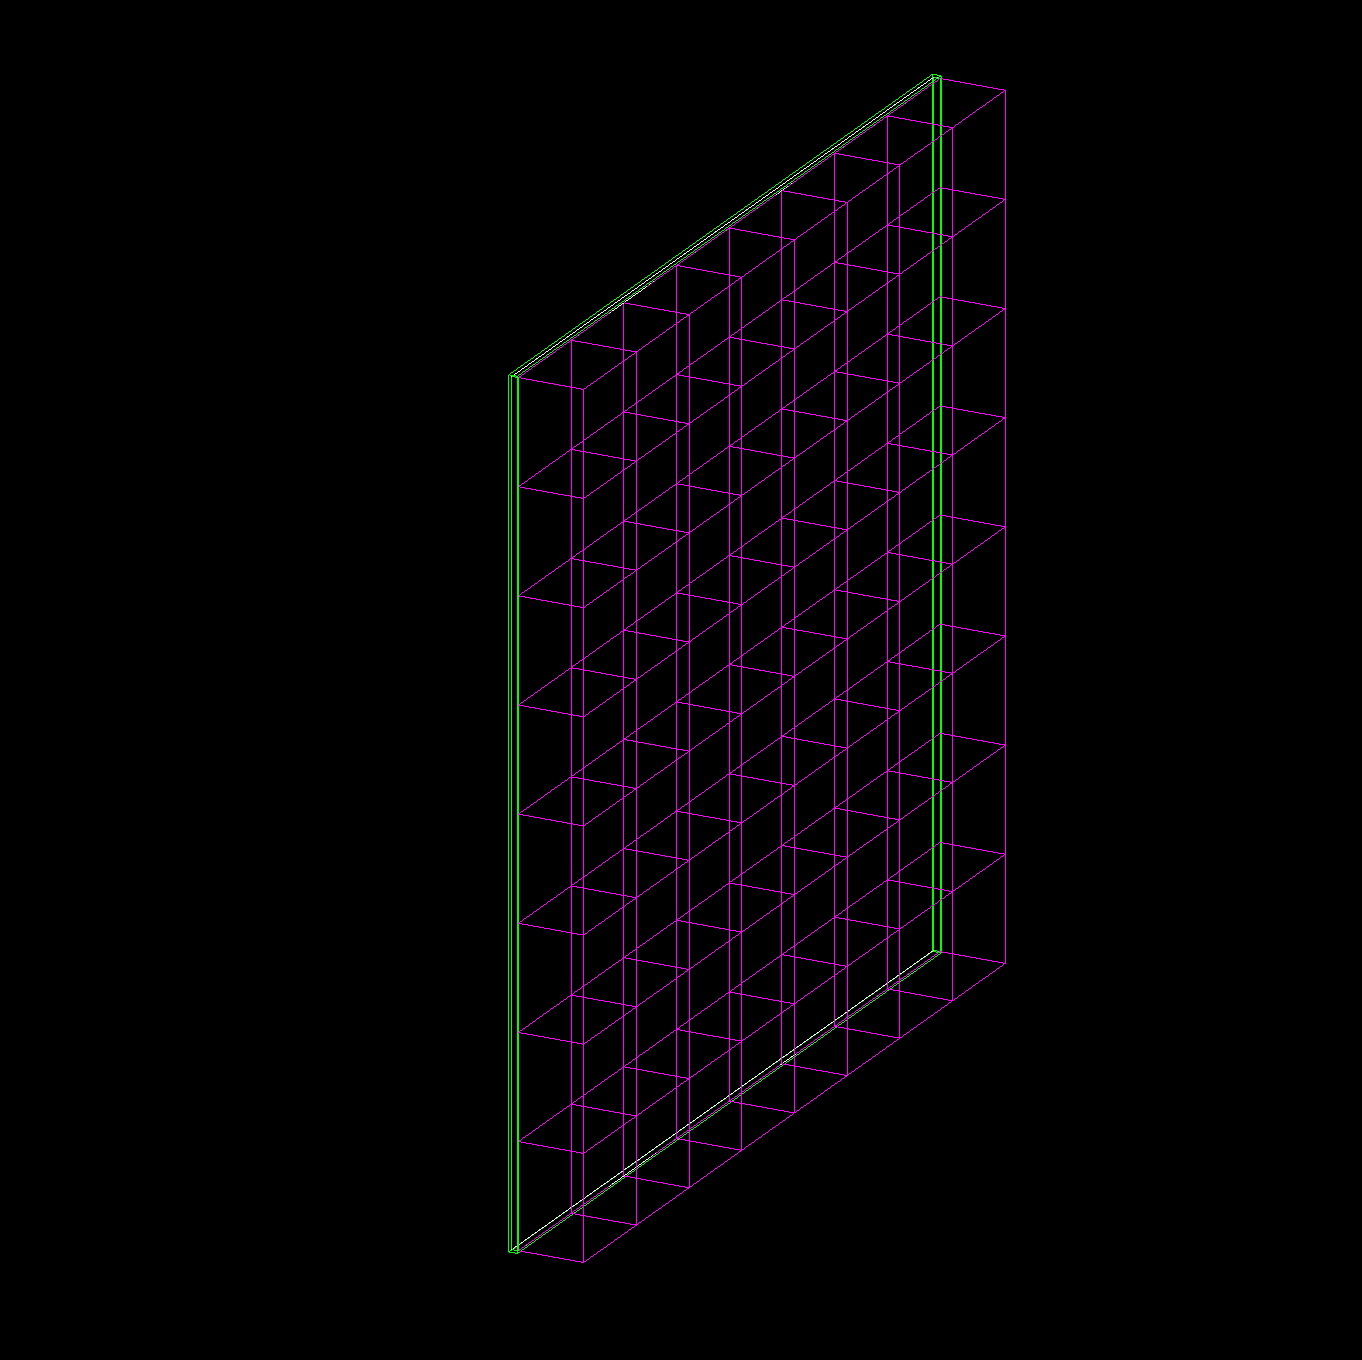
\includegraphics[width=0.48\textwidth, height=0.4\textheight]{images/monolithic_pixelarray.png}
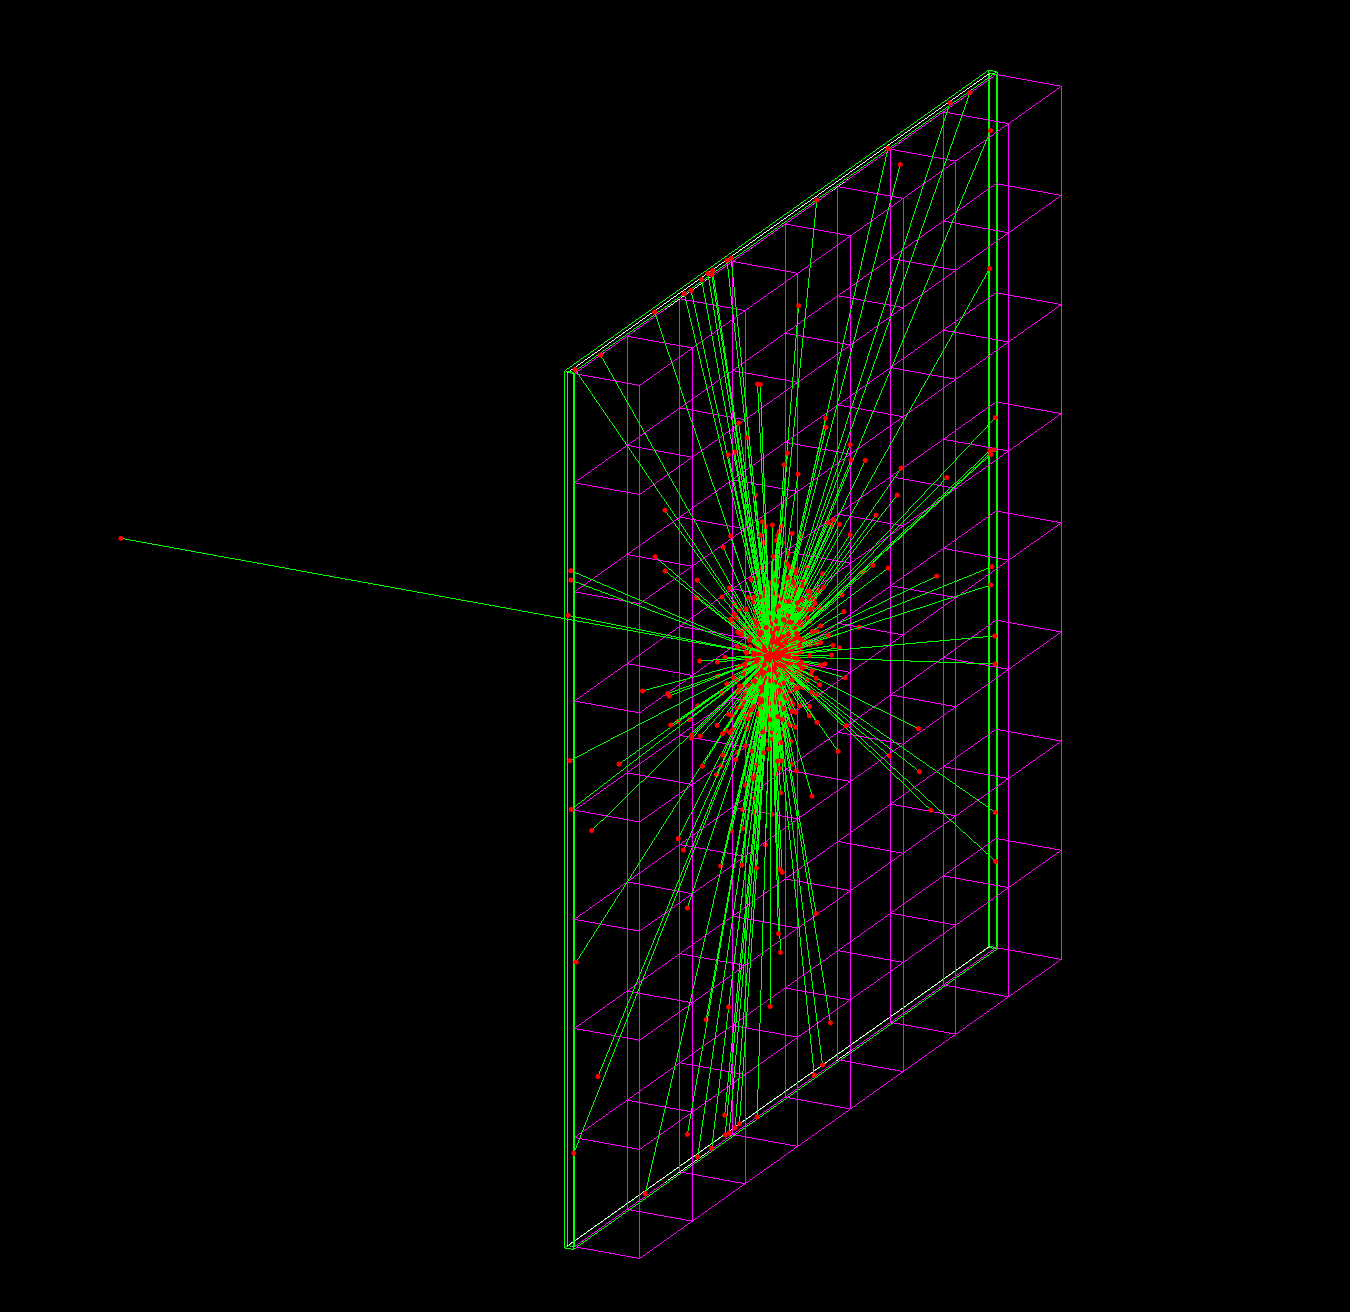
\includegraphics[width=0.48\textwidth, height=0.4\textheight]{images/monolithic_pixelarray1.png}
\end{frame}


\section{\scshape Results and Discussions}
% \begin{frame}
% \frametitle{Results: Light Collection Efficiency}
% % \scriptsize 
% To optimize scintillator parameters to maximize the light collection efficiency, the light collection efficiency is compared for different scintillator surface treatments and aspect ratios. \\
% \ \\

% \begin{columns}
% \begin{column}{0.5\textwidth}
% 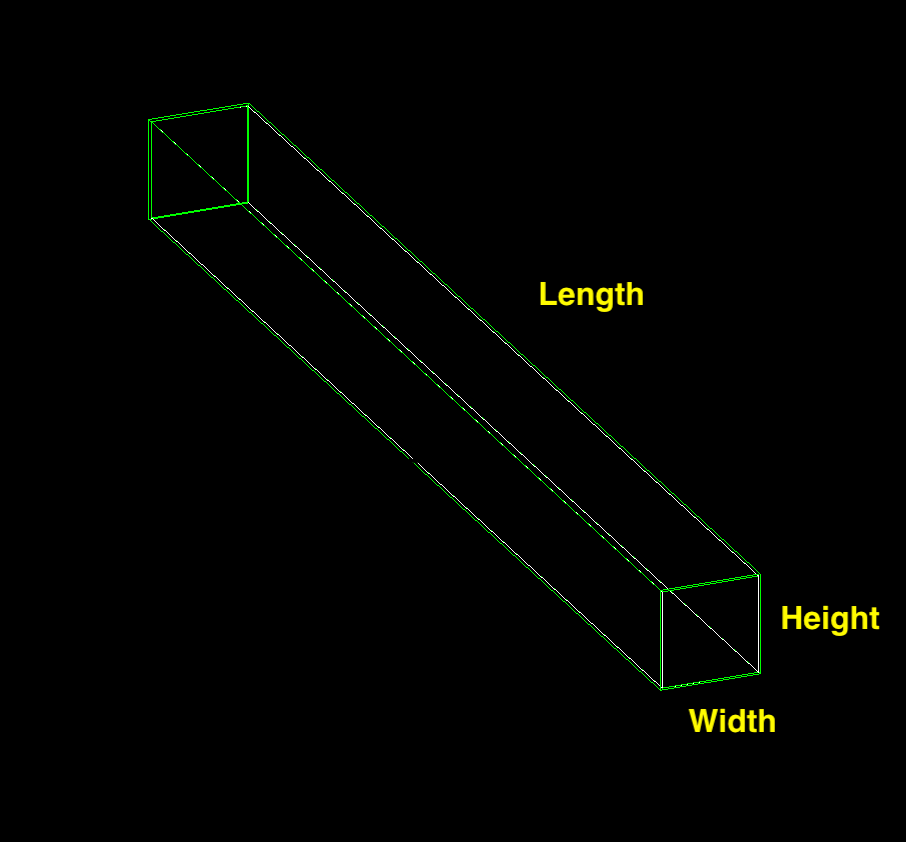
\includegraphics[width=\textwidth]{images/aspect_ratio.png}
% \end{column}
% \begin{column}{0.5\textwidth}
% The aspect ratio of a geometric shape is the ratio of its sizes in different dimensions. \\
% \ \\
% Here, we will talk about the aspect ratio of a cuboid (assume that width and height are of equal dimension)
% $$ aspect ~ratio = \frac{length}{width} $$ 
% \end{column}
% \end{columns}
% % 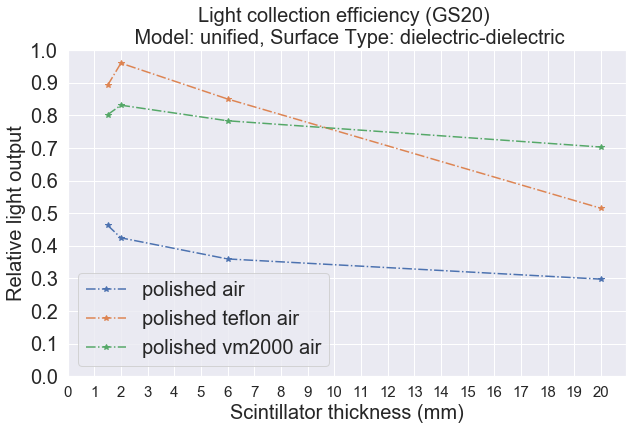
\includegraphics[width=0.49\textwidth, height=0.49\textheight]{images/gs20_lightyield_polished.png}
% % 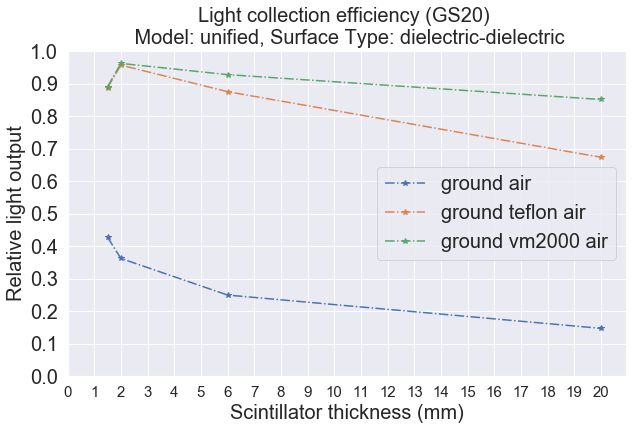
\includegraphics[width=0.49\textwidth, height=0.49\textheight]{images/gs20_lightyield_rough.png}
% % \scriptsize  \flushleft~~~~~~~~~~~~~~~~~~~~~ Polished crystal \hspace{4cm} Rough crystal 
% % The reflectivity specified in different types of reflection does not take into account the angular dependency in reflectivity.
% \end{frame}

% \begin{frame}
% \frametitle{Results: Validation Using Published Results}
% % \scriptsize 
% % To optimize scintillator parameters to maximize the light collection efficiency, the light collection efficiency is compared for different scintillator surface treatments and thicknesses. \\
% \centering
% 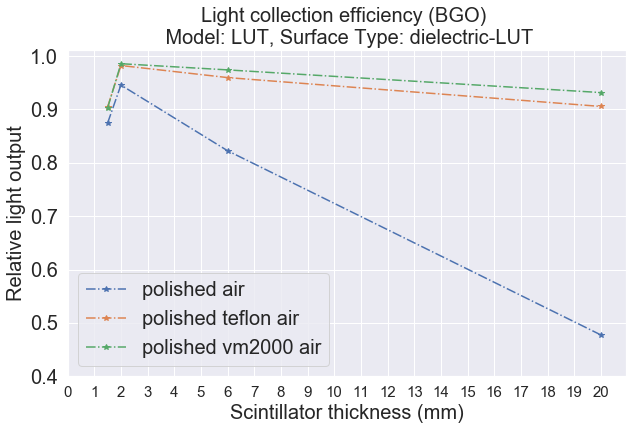
\includegraphics[width=0.49\textwidth, height=0.45\textheight]{images/bgo_lightyield_polished1.png}
% 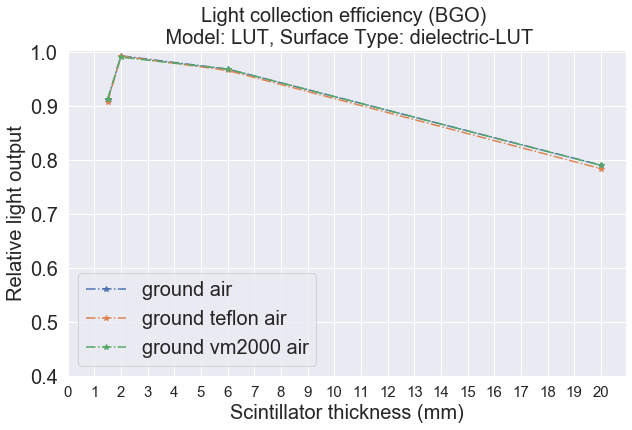
\includegraphics[width=0.49\textwidth, height=0.45\textheight]{images/bgo_lightyield_rough1.png}
% \scriptsize  \flushleft~~~~~~~~~~~~~~~~~~~~~ Polished crystal \hspace{4cm} Rough crystal
% \begin{block}{Findings}
% \begin{itemize}
%   \item For polished surfaces, having optical reflectors generally provides better light collection.
%   \item For rough surfaces, having reflectors does not necessary help with better light collection.
%   \item "Surface roughness proved to be the most important parameter when choosing crystal setup. The reflector choice was of less importance and of almost no consequence for rough-cut surfaces." \cite{janecek_moses_2008}
% \end{itemize}
% \end{block}
% % 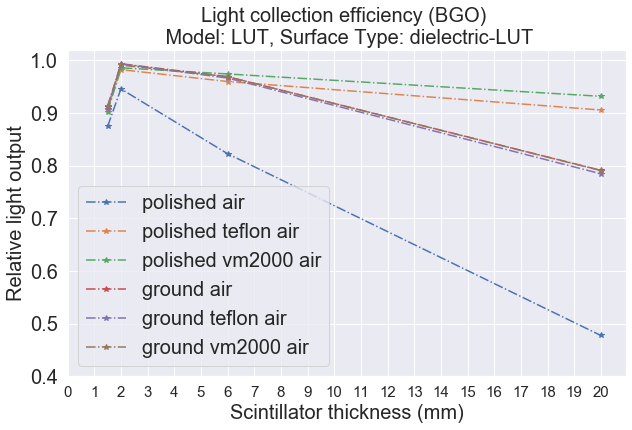
\includegraphics[width=0.49\textwidth, height=0.45\textheight]{images/BGO_lightyield_LUT1.png}

% % 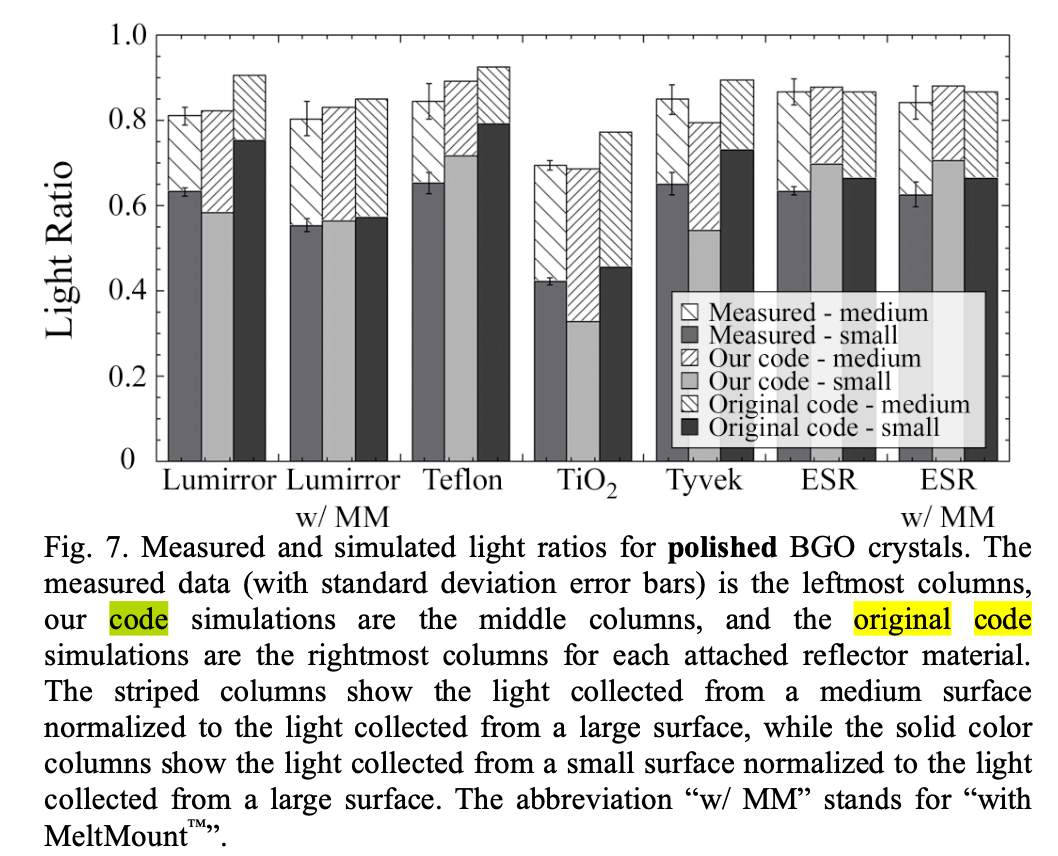
\includegraphics[width=0.49\textwidth, height=0.45\textheight]{images/bgo_polished.png}
% % 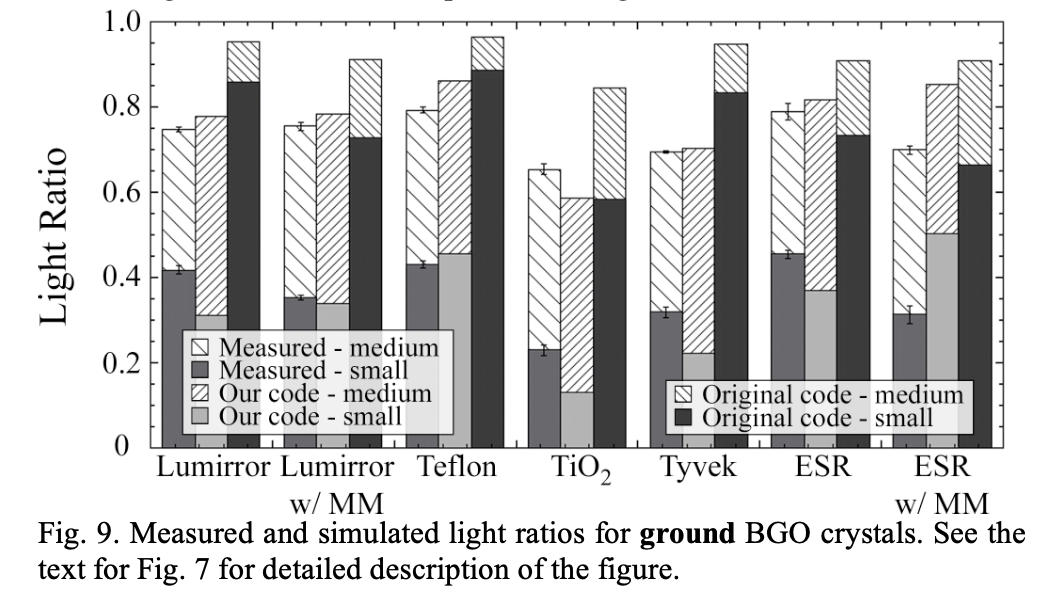
\includegraphics[width=0.49\textwidth, height=0.45\textheight]{images/bgo_rough.png}
% % The reflectivity specified in different types of reflection does not take into account the angular dependency in reflectivity.
% \end{frame}

% \begin{frame}
% \scriptsize
% Below shows the comparison between experimental measurements ($Measured$), simulated results using LUT ($Our ~code$)and Geant4 unified model ($Original~code$) \cite{janecek_2012}. \\
% The BGO crystal used has a dimension of 3 $\times$ 10 $\times$ 30 mm$^3$.
% \scriptsize  \flushleft~~~~~~~~~~~~~~~~~~~~~ Polished crystal \hspace{4cm} Rough crystal
% 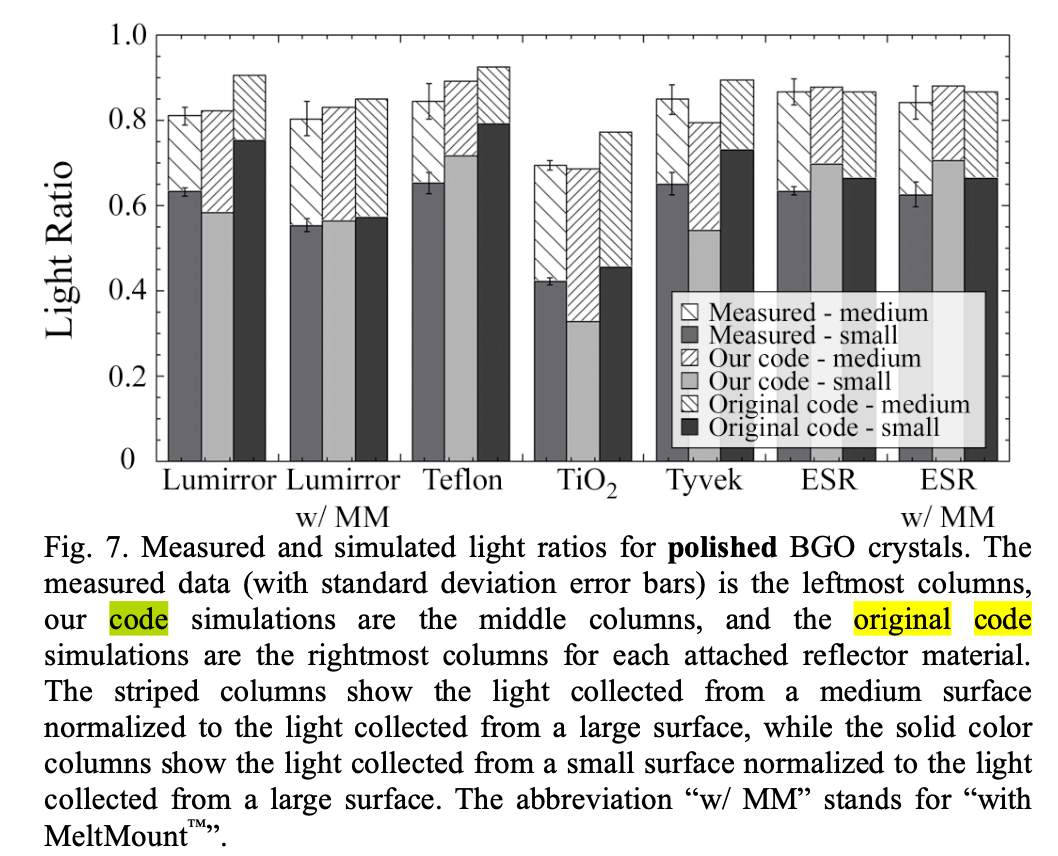
\includegraphics[width=0.49\textwidth, height=0.4\textheight]{images/bgo_polished.png}
% 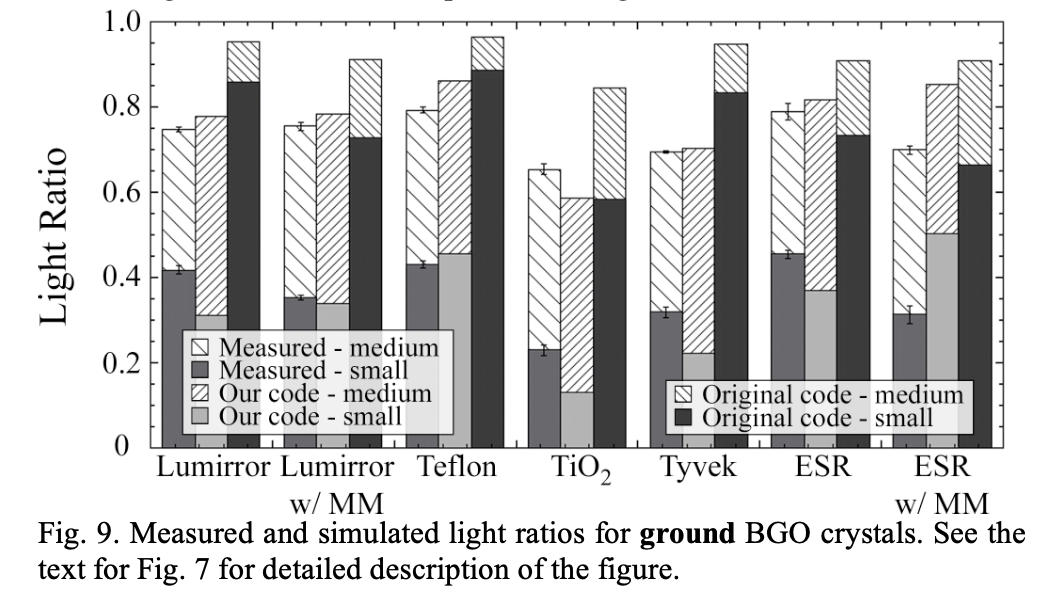
\includegraphics[width=0.49\textwidth, height=0.4\textheight]{images/bgo_rough.png}
% 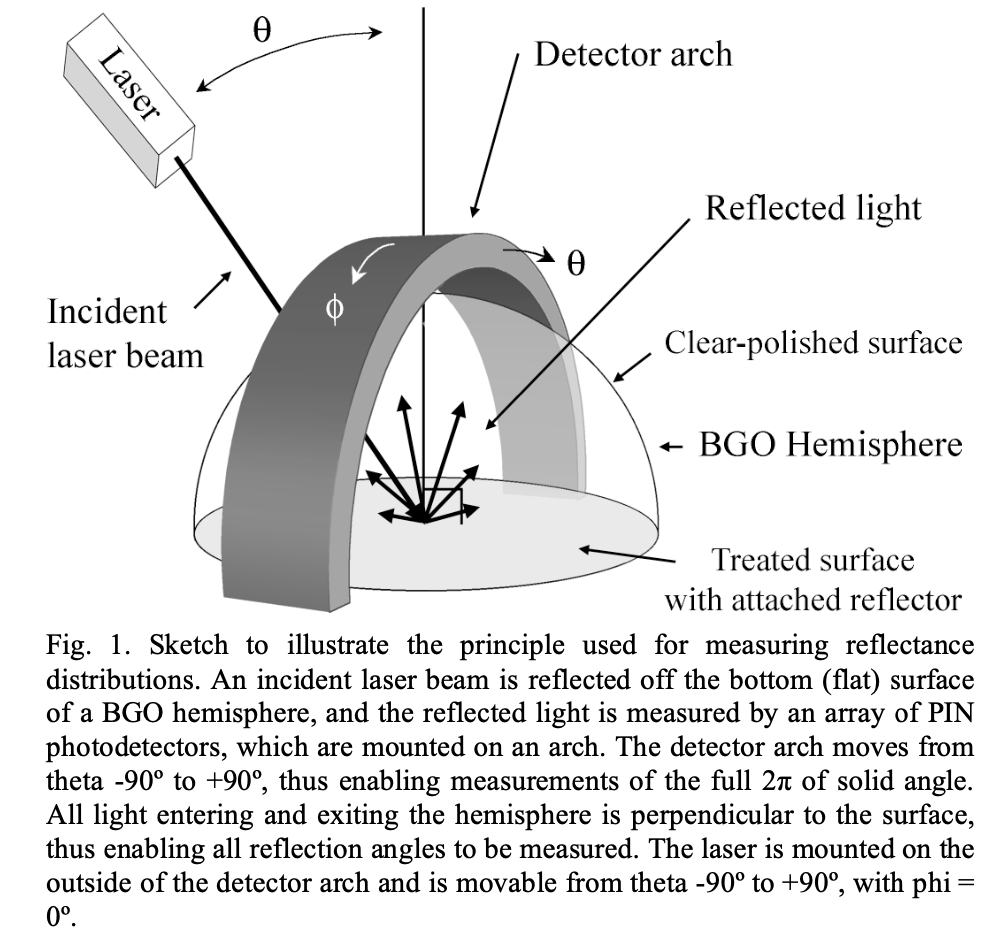
\includegraphics[width=0.49\textwidth, height=0.4\textheight]{images/bgo_setup.png}
% 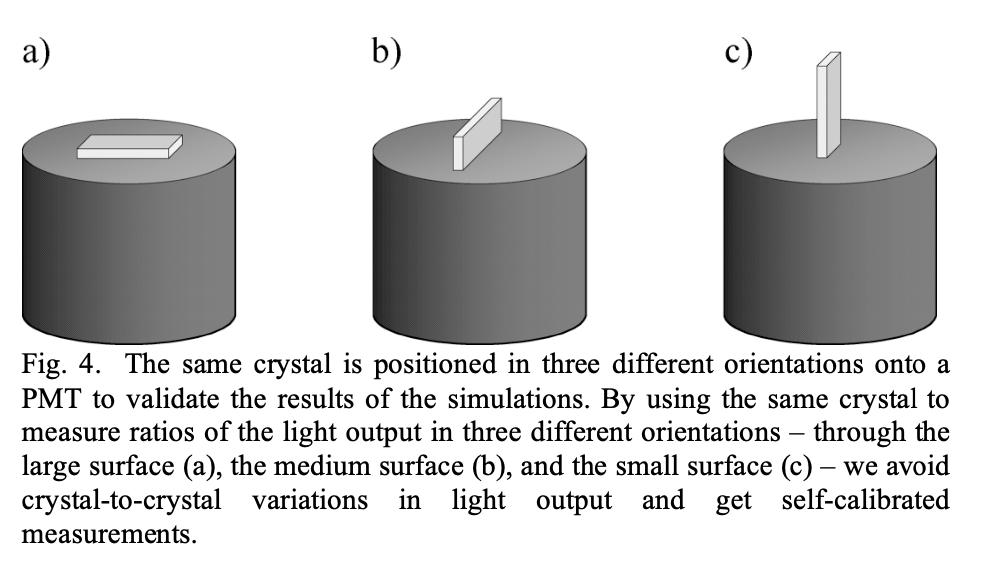
\includegraphics[width=0.49\textwidth, height=0.4\textheight]{images/bgo_orientation.png}
% \end{frame}

\begin{frame}
\begin{columns}
\begin{column}{0.6\textwidth}
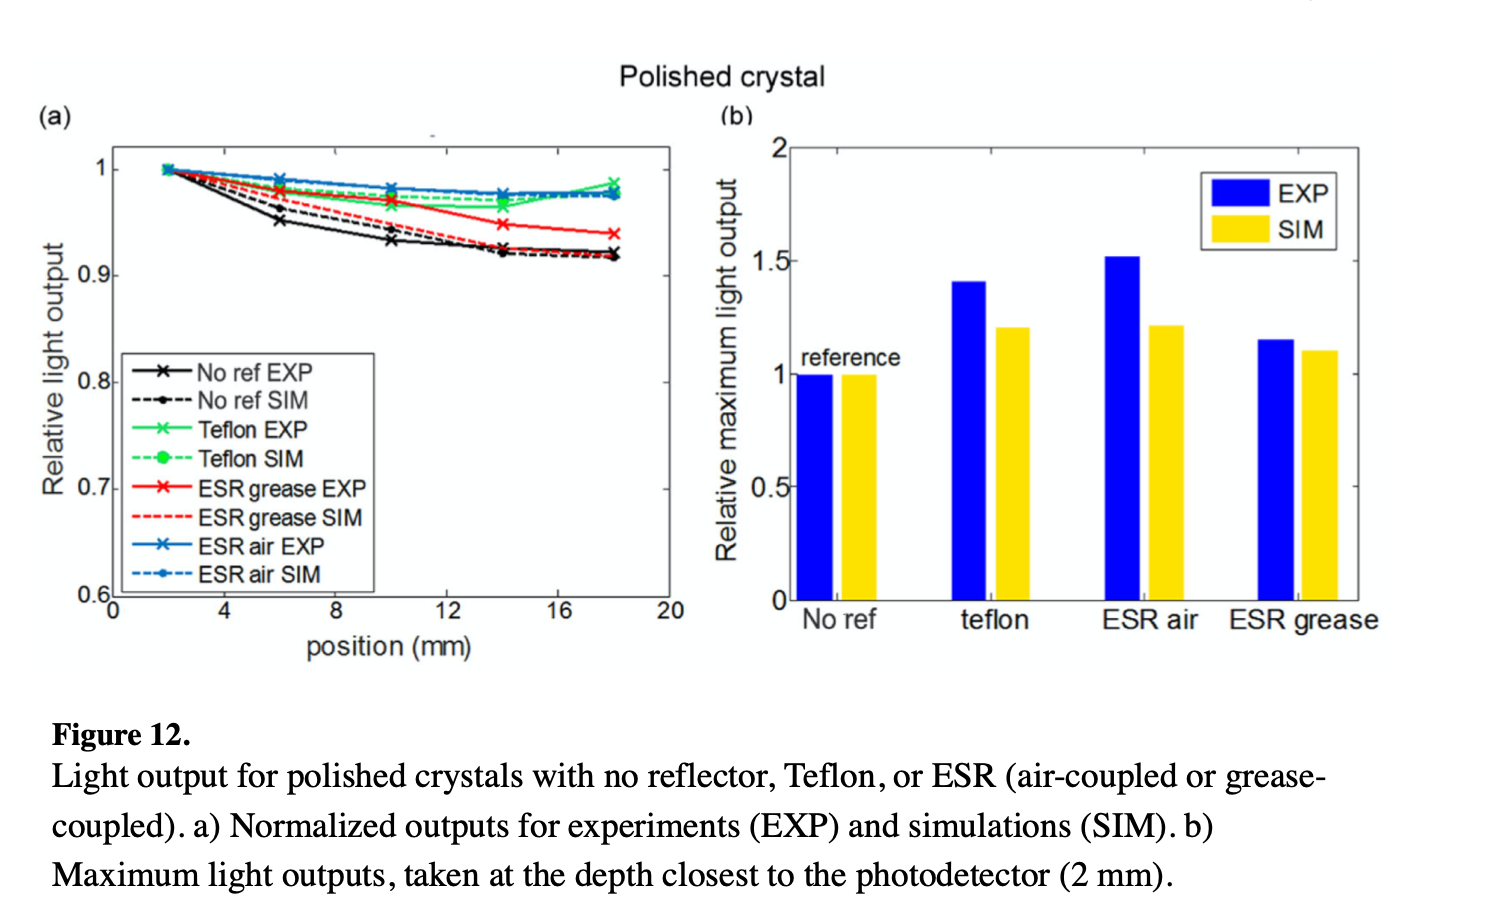
\includegraphics[width=\textwidth, height=0.49\textheight]{images/lyso_polished.png}
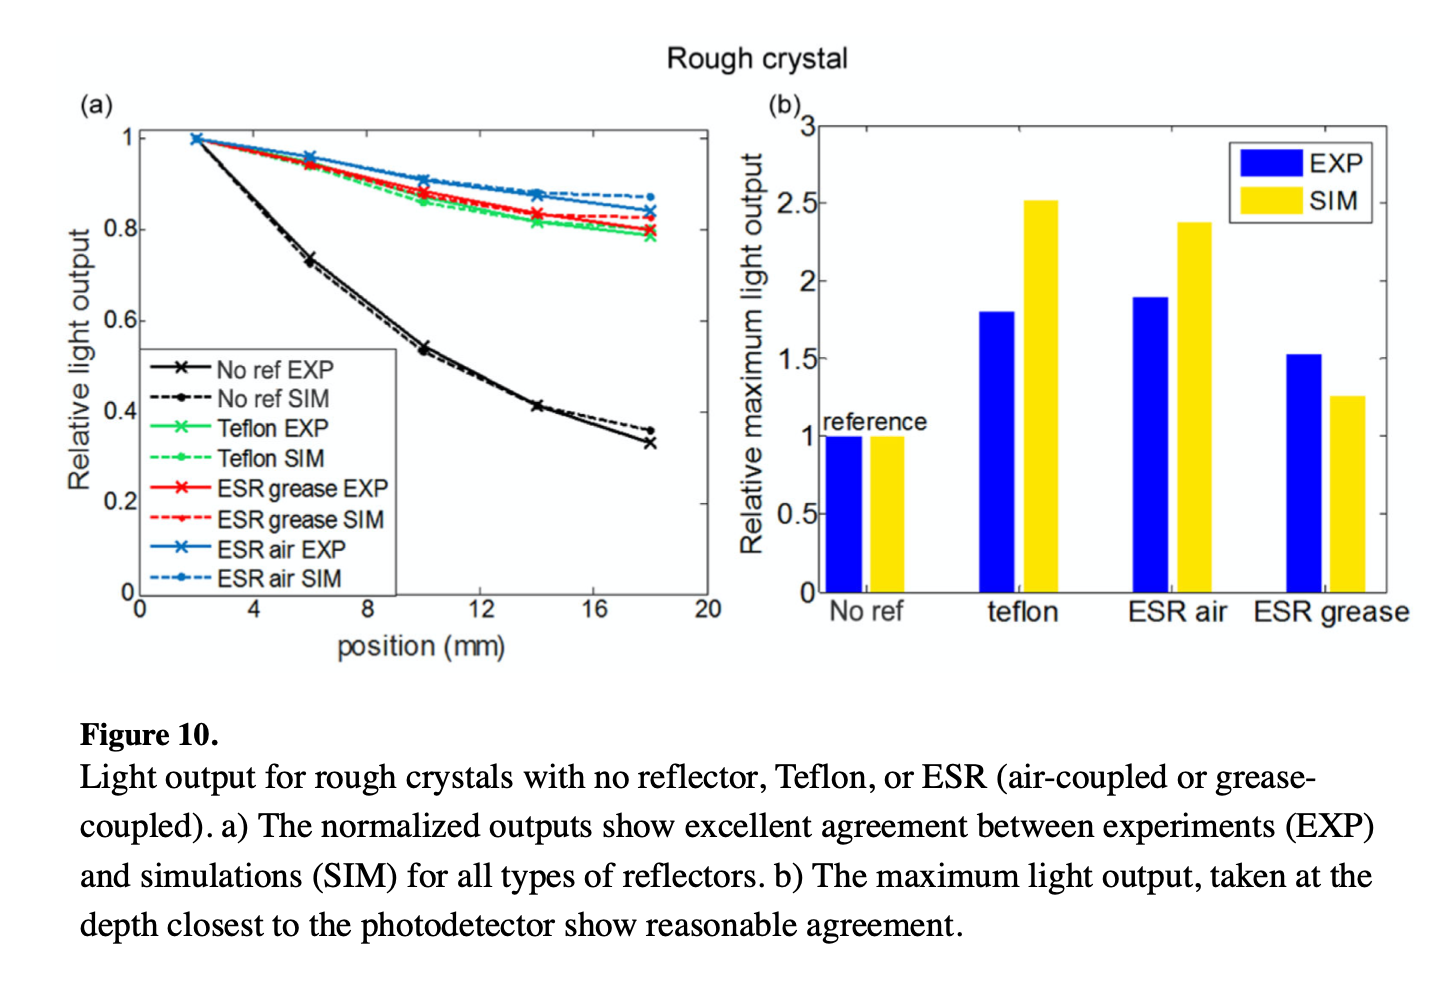
\includegraphics[width=0.95\textwidth, height=0.49\textheight]{images/lyso_rough.png}
\end{column}
\begin{column}{0.39\textwidth}
\scriptsize
The LYSO crystal used has a dimension of 3 $\times$ 3 $\times$ 20 mm$^3$. These measurements were conducted by another publication.\cite{roncali_stockhoff_cherry_2017}
% Comparison between simulated results and experimental measurements showed consistent results with the previous publication. 

\begin{block}{Findings}
\begin{itemize}
\item Showed consistent results that thicker scintillators (larger aspect ratio) has better light collection with the coupling of optical reflectors to polished surfaces. 
\item It was also measured that as the thinner scintillators (smaller aspect ratio) collect light better in rough surfaces. 
\item However, it showed that coupling of optical reflectors makes a different in light collection for rough surfaces. 
\end{itemize}
\end{block}
\end{column}
\end{columns}
\end{frame}


\begin{frame}
\frametitle{Results: Light Sharing / Crosstalk }
\end{frame}

\section{\scshape Conclusion and Future Work}
\begin{frame}
\frametitle{Conclusion}
\end{frame}

\begin{frame}
\frametitle{Future Work}
Measure experimental data
Measure our own LUT 
\end{frame}

\begin{frame}
\frametitle{Acknowledgement}
Most of the framework can be obtained from Dr. Micah Folsom's public Github repository. (https://github.com/micahfolsom/mgg4)
\end{frame}

\frame[noframenumbering, plain]{\frametitle{References}
\tiny{\bibliographystyle{plain}}
\bibliography{bib/bib}
}

\appendix

\section{Backup Slides}
\begin{frame}[noframenumbering, plain]
\frametitle{Equations}
Snell's law:
$$ n_i ~sin(\theta_i) = n_t ~sin(\theta_t) $$

Critical angle:
$$ \theta_c = sin^{-1}(n_t/n_i) $$
\end{frame}

\begin{frame}
\frametitle{Relevant Published Data}
\begin{block}{Scintillator crystal without any reflectors: }
\centering \scriptsize
\begin{tabular}{ c | c c c}
& GS20 & LYSO & BGO \\
\hline
Refractive Index & 1.55 & 1.81 & 2.15 \\
Critical angle ($^o$) & 40.18 & 33.53 & 26.23 \\ 
Wavelength at maximum emission (nm) & 395 & 420 & 480 \\
\end{tabular}
\end{block}

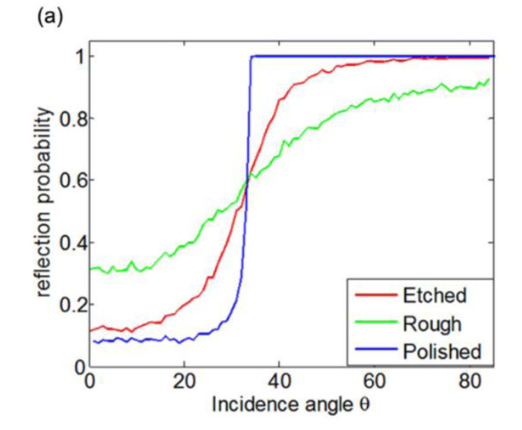
\includegraphics[width=0.49\textwidth, height=0.45\textheight]{images/LYSO_reflectivity_angular_distribution.png}
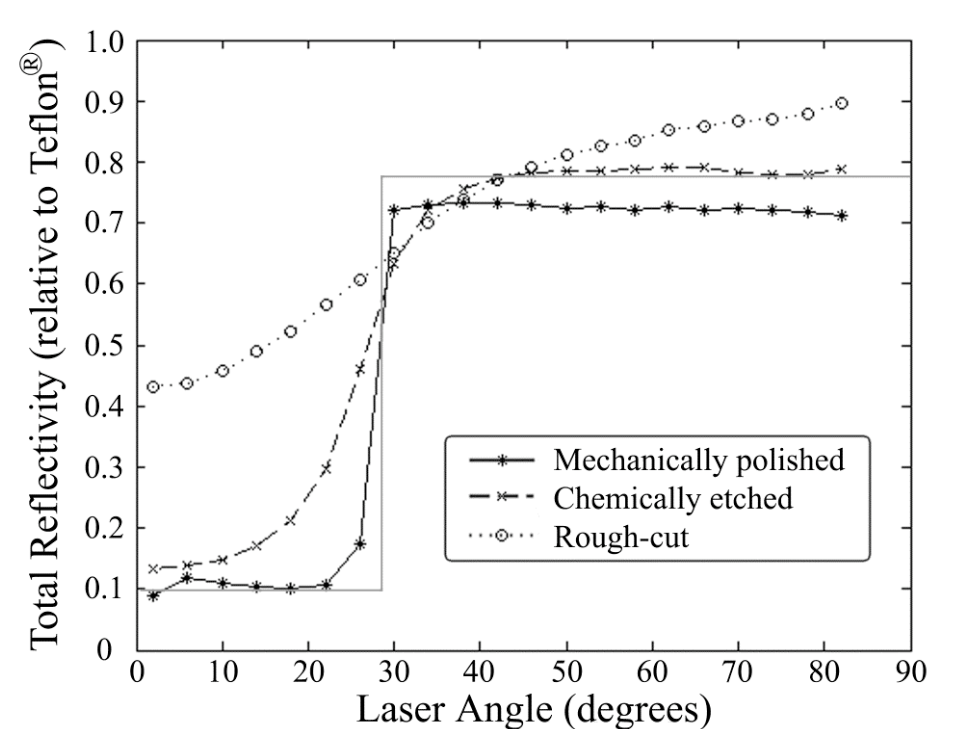
\includegraphics[width=0.49\textwidth, height=0.45\textheight]{images/BGO_reflectivity_angular_distribution.png}
\scriptsize \flushleft~~~~~~~~~~~~~~~~~~~~~~~~ LYSO \cite{roncali_stockhoff_cherry_2017} \hspace{5cm} BGO \cite{janecek_moses_2010} \hspace{3cm}
\end{frame}

\begin{frame}
\frametitle{Relevant Published Data}
Several reflectors exhibits "cut-offs" for the reflectivity for shorter wavelengths, such as TiO$_2$ (420 nm) and ESR film (395 nm). \cite{janecek_2012} \\
\ \\
Reflectivity curve as a function of wavelengths: \\
\ \\
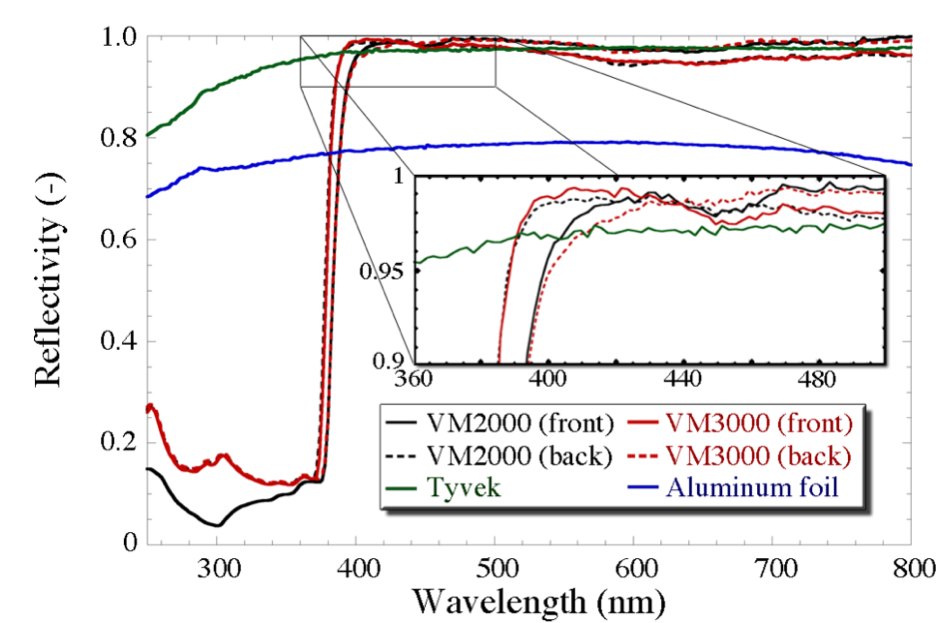
\includegraphics[width=0.49\textwidth, height=0.45\textheight]{images/vm2000_reflectivity_curve1}
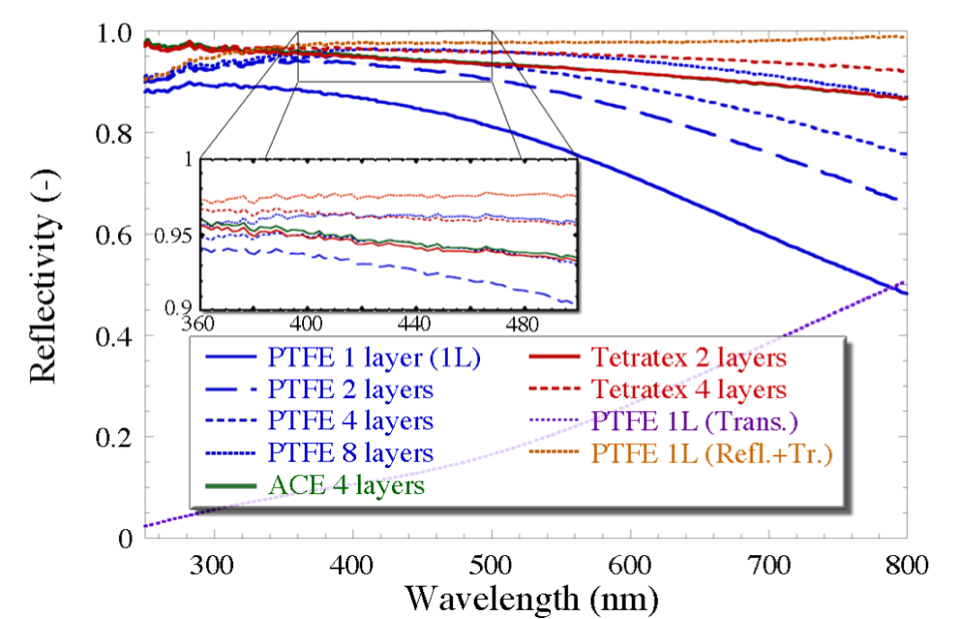
\includegraphics[width=0.49\textwidth, height=0.45\textheight]{images/teflon_reflectivity_curve1}
\scriptsize \flushleft~~~~~~~~~~~~~~~~~~~~~~~ VM2000 \cite{janecek_2012}  \hspace{5cm} Teflon \cite{janecek_2012} \hspace{3cm}
\end{frame}


\end{document}